

\tikzset{every picture/.style={line width=0.75pt}} %set default line width to 0.75pt        

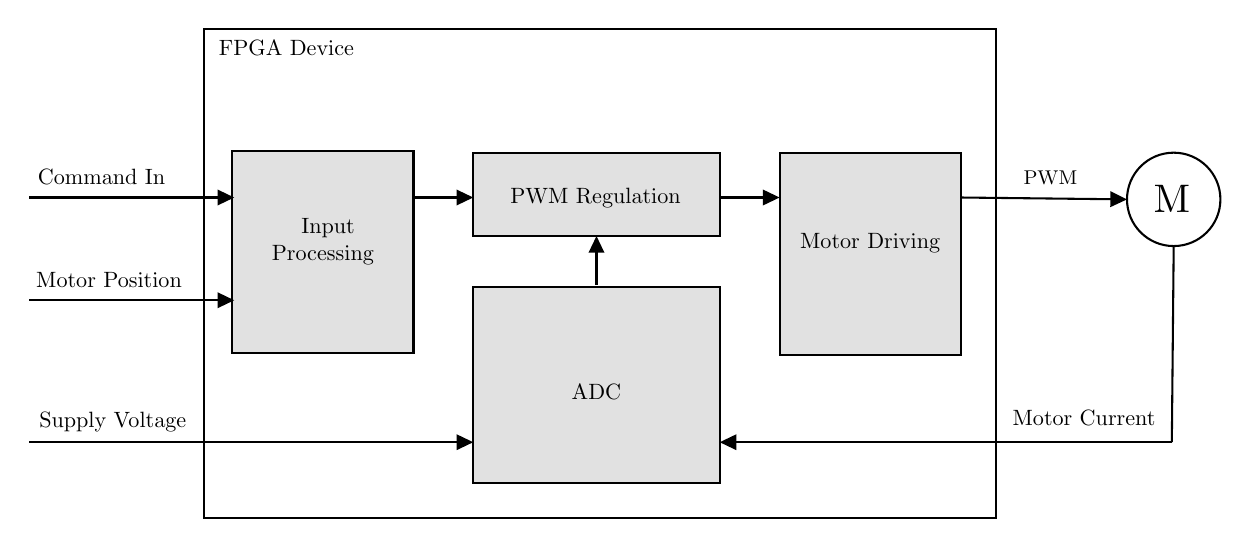
\begin{tikzpicture}[x=0.75pt,y=0.75pt,yscale=-0.9,xscale=0.9]
%uncomment if require: \path (0,290.6363525390625); %set diagram left start at 0, and has height of 290.6363525390625

%Shape: Circle [id:dp37060167234059627] 
\draw   (602,107) .. controls (602,93.19) and (613.19,82) .. (627,82) .. controls (640.81,82) and (652,93.19) .. (652,107) .. controls (652,120.81) and (640.81,132) .. (627,132) .. controls (613.19,132) and (602,120.81) .. (602,107) -- cycle ;

%Straight Lines [id:da8457845643324124] 
\draw    (513.05,106) -- (599,106.97) ;
\draw [shift={(602,107)}, rotate = 180.64] [fill={rgb, 255:red, 0; green, 0; blue, 0 }  ][line width=0.08]  [draw opacity=0] (8.93,-4.29) -- (0,0) -- (8.93,4.29) -- cycle    ;

%Shape: Rectangle [id:dp9895913562419061] 
\draw  [fill={rgb, 255:red, 225; green, 225; blue, 225 }  ,fill opacity=1 ] (416.05,82) -- (513.05,82) -- (513.05,190.36) -- (416.05,190.36) -- cycle ;
%Straight Lines [id:da89362591639862] 
\draw    (626,237) -- (387,237) ;
\draw [shift={(384,237)}, rotate = 360] [fill={rgb, 255:red, 0; green, 0; blue, 0 }  ][line width=0.08]  [draw opacity=0] (8.93,-4.29) -- (0,0) -- (8.93,4.29) -- cycle    ;

%Straight Lines [id:da3647004512136063] 
\draw    (626,237) -- (627,132) ;


%Shape: Rectangle [id:dp22253882061890917] 
\draw   (108.05,15.64) -- (532.05,15.64) -- (532.05,277.64) -- (108.05,277.64) -- cycle ;
%Straight Lines [id:da4479460701262754] 
\draw    (384.64,106) -- (413,106) ;
\draw [shift={(416,106)}, rotate = 180] [fill={rgb, 255:red, 0; green, 0; blue, 0 }  ][line width=0.08]  [draw opacity=0] (8.93,-4.29) -- (0,0) -- (8.93,4.29) -- cycle    ;

%Shape: Rectangle [id:dp7862653443183867] 
\draw  [fill={rgb, 255:red, 225; green, 225; blue, 225 }  ,fill opacity=1 ] (252,82) -- (384,82) -- (384,126.64) -- (252,126.64) -- cycle ;
%Shape: Rectangle [id:dp8459838496523577] 
\draw  [fill={rgb, 255:red, 225; green, 225; blue, 225 }  ,fill opacity=1 ] (123.05,81) -- (220.05,81) -- (220.05,189.36) -- (123.05,189.36) -- cycle ;
%Straight Lines [id:da5317523796080506] 
\draw    (318,129.64) -- (318,152.64) ;

\draw [shift={(318,126.64)}, rotate = 90] [fill={rgb, 255:red, 0; green, 0; blue, 0 }  ][line width=0.08]  [draw opacity=0] (8.93,-4.29) -- (0,0) -- (8.93,4.29) -- cycle    ;
%Straight Lines [id:da8756486664401073] 
\draw    (220.64,106) -- (249,106) ;
\draw [shift={(252,106)}, rotate = 180] [fill={rgb, 255:red, 0; green, 0; blue, 0 }  ][line width=0.08]  [draw opacity=0] (8.93,-4.29) -- (0,0) -- (8.93,4.29) -- cycle    ;

%Shape: Rectangle [id:dp2661938237798891] 
\draw  [fill={rgb, 255:red, 225; green, 225; blue, 225 }  ,fill opacity=1 ] (252,154) -- (384,154) -- (384,258.64) -- (252,258.64) -- cycle ;
%Straight Lines [id:da7659205141917105] 
\draw    (249,237) -- (14.05,237) ;

\draw [shift={(252,237)}, rotate = 180] [fill={rgb, 255:red, 0; green, 0; blue, 0 }  ][line width=0.08]  [draw opacity=0] (8.93,-4.29) -- (0,0) -- (8.93,4.29) -- cycle    ;
%Straight Lines [id:da5160015319494151] 
\draw    (121.05,161) -- (14.05,161) ;

\draw [shift={(124.05,161)}, rotate = 180] [fill={rgb, 255:red, 0; green, 0; blue, 0 }  ][line width=0.08]  [draw opacity=0] (8.93,-4.29) -- (0,0) -- (8.93,4.29) -- cycle    ;
%Straight Lines [id:da10479838194944624] 
\draw    (121.05,106) -- (14.05,106) ;

\draw [shift={(124.05,106)}, rotate = 180] [fill={rgb, 255:red, 0; green, 0; blue, 0 }  ][line width=0.08]  [draw opacity=0] (8.93,-4.29) -- (0,0) -- (8.93,4.29) -- cycle    ;

% Text Node
\draw (561,95.5) node  [scale=0.8] [align=left] {{\small PWM}};
% Text Node
\draw (626,107) node  [scale=1.44] [align=left] {M};
% Text Node
\draw (464.52,130.62) node  [scale=0.8] [align=left] {Motor Driving};
% Text Node
\draw (318,210) node  [scale=0.8] [align=left] {ADC};
% Text Node
\draw (579.02,224) node  [scale=0.8] [align=left] {Motor Current};
% Text Node
\draw (317.52,106) node  [scale=0.8] [align=left] {PWM Regulation};
% Text Node
\draw (171.52,129.62) node  [scale=0.8] [align=left] { \ \ \ \ Input \\Processing};
% Text Node
\draw (53.05,95) node  [scale=0.8] [align=left] {Command In};
% Text Node
\draw (57.05,150) node  [scale=0.8] [align=left] {Motor Position};
% Text Node
\draw (59.05,226) node  [scale=0.8] [align=left] {Supply Voltage};
% Text Node
\draw (152.05,26) node  [scale=0.8] [align=left] {FPGA Device};


\end{tikzpicture}
